\chapter{Estimador analógico} \chapterlabel{Informe/5-EstimadorAnalogico} \label{cap:Estimador Analogico}

Para que la placa de control pueda mantener la distancia de separación $Y_{g}$ es necesario conocer su valor para luego actuar en consecuencia. Si bien se podrían utilizar sensores  especializados para ello, para este proyecto se optó por medirla de manera indirecta a partir de la pendiente de la corriente que circula por el electroimán. De esta forma, se logran aplicar conceptos de estimación de variables, aprendidos durante la carrera. 

En este capítulo se detalla la estrategia utilizada para realizar la estimación de posición a partir de la corriente del electroimán, junto con el diseño circuital y sus respectivas simulaciones. Finalmente se obtiene una función transferencia del bloque estimador que será luego utilizada para el diseño del compensador analógico.

\section{Análisis de la estimación}

Como se analizó en el capítulo 3, para controlar el valor medio de la corriente se utiliza una fuente conmutada que alterna la polaridad de la tensión aplicada al electroimán. Esto genera una onda de corriente triangular superpuesta al valor medio deseado, cuyas pendientes de crecimiento y de decrecimiento contienen información de la distancia de separación de entrehierro. Con esta información se decidió realizar una estimación de la distancia a partir de la medición de la pendiente de la onda triangular de la corriente.

En la sección 3.2.1 se obtuvo una ecuación que relaciona la pendiente de la corriente con la distancia de entrehierro, en función de constantes del sistema. Si bien este resultado es correcto, para tener una mejor aproximación se realiza el cálculo de la ecuación 3.7 utilizando la expresión de inductancia linealizada (calculada en el capítulo 2).

\begin{equation} \label{eq_inductancia_lineal_teorica}
	L(y_{g})=-2.2089*Y_{g}+0.0177\:Hy
\end{equation}

Utilizando esta inductancia en la ecuación 3.7 se obtiene una expresión no lineal, que se vuelve a linealizar y se obtiene:

\begin{equation} \label{eq_di-dt_lineal}
	{\left|\frac{{dI}_L}{dt}\right|}_{Lineal}=\ 194690\ *\ Y_g\:[m]+676\:A/s
\end{equation}

Por lo tanto, al despejar la distancia de separación se obtiene:
\colorbox{red}{Despejar Yg}

\begin{equation} \label{eq_Yg_despejada}
	{\left|\frac{{dI}_L}{dt}\right|}_{Lineal}=\ 194690\ *\ Y_g\:[m]+676\:A/s
\end{equation}

Al observar la expresión \ref{eq_Yg_despejada}, es necesario diseñar un circuito que pueda obtener el módulo de la derivada de la corriente. Esto se puede implementar circuitalmente a través de dos etapas: un derivador y un rectificador.

Además se decidió agregar un LPF luego del rectificador para reducir las frecuencias no deseadas introducidas por el cambio de signo de la pendiente, las cuales generan saltos sobre un punto de operación en la tensión de salida del derivador.

A continuación se describe la implementación circuital de cada uno de ellos.

{
	%Por lo tanto, en esta capítulo/sección.. se aborda el análisis de la implementación…
	
	%En el capítulo 3 se analizó la forma de onda resultante de la corriente del electroimán al ser excitado con una fuente conmutada. Esta resulta en una onda triangular con un valor medio deseado, cuya pendiente de crecimiento y de decrecimiento varía proporcionalmente con distancia de separación de entrehierro. A partir de esto, se decidió realizar una estimación de la misma a partir de la medición de la pendiente de la onda triangular de la corriente.
}

\section{Modelo circuital del estimador de posición}

Para poder obtener $\left|\frac{{dI}_L}{dt}\right|$ se utiliza un circuito derivador con un amplificador operacional como se observa en la figura  \ref{fig:img_Circuito-derivador}.

\begin{figure}[H]
	\centering
	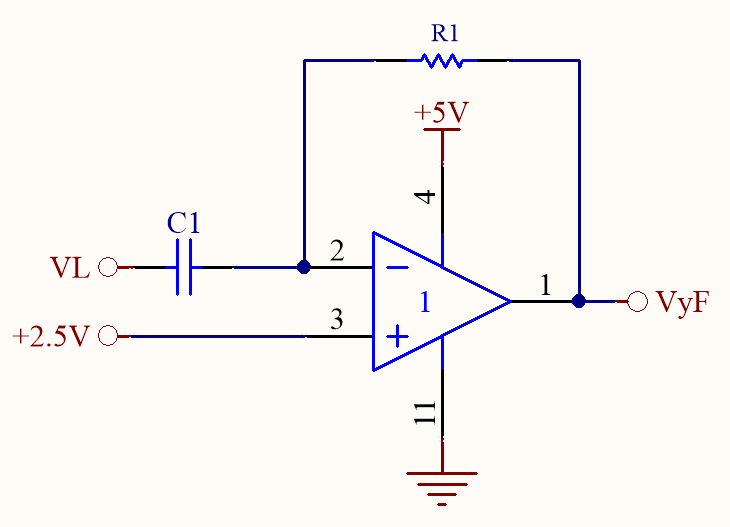
\includegraphics[scale=0.6]{Circuito-derivador.png}
	\caption{Circuito derivador.}
	\label{fig:img_Circuito-derivador}
\end{figure}

La salida del circuito $V_{yf}(t)$ ante una entrada $V_L$ es:

\begin{equation} \label{eq_vyf1}
	V_{yf}(t)\ =\ 2.5V\ -\ \frac{dV_{iL}}{dt}*C_1*R_1
\end{equation}

Teniendo en cuenta que $V_{iL}=K_h*I_L$, es la salida del sensor de efecto Hall con $K_h$ como su ganancia (seccion XD), se obtiene: 

\begin{equation} \label{eq_vyf2}
	V_{yf}(t)\ =2.5\:V\ -\frac{dI_L}{dt}*K_h*C_1*R_1
\end{equation}

Para evitar una saturación de la salida del derivador y teniendo en cuenta que $V_{yf}(t)$ presenta variaciones alrededor del \textsl{set-point} de $2.5\:V$ se debe cumplir que:

\begin{equation} \label{eq_vyf3}
	\left|-\frac{dI_L}{dt}*K_h*C_1*R_1\right|\ \le 2.5\:V
\end{equation}

Por lo tanto, con la ecuación \ref{eq_derivadaAproximacion} y \ref{eq_vyf3}:

\begin{equation} \label{eq_condicionC1-R1}
	C_1*R_1\le\frac{2.5\ \:V\ *L_{min}}{V_{BUS}*K_h}
\end{equation}

Con $L_{min}= L(5\: mm) + L_{\infty}= 14.9\: mHy$ se obtiene: 

\begin{equation} \label{eq_condicionC1-R1-2}
	C_1*R_1\le\ 29.1\ ms
\end{equation}

El derivador tiene como salida una onda pulsada, cuyo nivel superior es proporcional a la pendiente de bajada de la corriente en el electroimán, y el nivel inferior es proporcional a la pendiente de subida.

Para los cálculos se utilizó $\tau = C_1*R_1= 25\:ms$, para dar un margen y evitar la saturación del amplificador operacional.  

Con la ecuación \ref{eq_di-dt_lineal} y \ref{eq_vyf2}, y con una variación en torno a $2.5\:V$ se obtiene:


\begin{equation} \label{eq_Vyf-lineal}
	Vyf(Y_g)\ =\ |K_h*C_1*R_1*dI_L/dt)|\ +2.5\:V=0.2595*Y_g+3.4\:V
\end{equation}

Se puede observar en la tabla \ref{tab_Vyf_vs_y} que, para los posibles valores en los que el electroimán trabaja, el estimador posee un rango de salida ${\mathit{\Delta}{Vyf}_{Lineal}}(5\:mm-2\:mm)= 0.78\:V$.

\begin{table}[H]
	\begin{center}
		\begin{tabular}{| c | c |}
			\hline
			$Y_g[\:mm]$ & ${Vyf(Y_g)}_{Lineal} [\:V]$\\ \hline
			2 & 3.92 \\ \hline 
			3 & 4.18 \\ \hline 
			4 & 4.44 \\ \hline 
			5 & 4.7 \\ \hline 
		\end{tabular}
		\caption{$V_{yf}$ en función de la posición.}
		\label{tab_Vyf_vs_y}
	\end{center}
\end{table}

\subsection{Elección de Amplificador Operacional}

Para el diseño del derivador es necesario escoger de forma adecuada un amplificador operacional que permita mantener características derivativas en toda la banda de interés.

Dado que la forma de onda triangular que se desea derivar posee una frecuencia fundamental de 2 KHz es necesario que el amplificador operacional seleccionado posea un ancho de banda y una ganancia suficiente que permita el diseño de un derivador con características derivativas hasta al menos la quinta armónica de dicha frecuencia que es de $2KHz*5=10 KHz$.

Se escogió el MCP660 el cual cumple con las características mencionadas anteriormente.El integrado posee una ganancia continua de 130 dB, y un polo en 20 Hz. Además se destaca su slew rate de 32 V/us.

\subsection{Circuito del derivador compensado}

Puesto que los circuitos derivadores pueden presentar inestabilidad a alta frecuencia, es necesario compensarlos mediante el agregado de una resistencia en serie al capacitor, para que genere un cero en la transferencia de realimentación (ecuación \ref{eq_Aw_2}), como se observa en la figura  \ref{fig:img_Circuito_derivador_compensado}.

\begin{figure}[H]
	\centering
	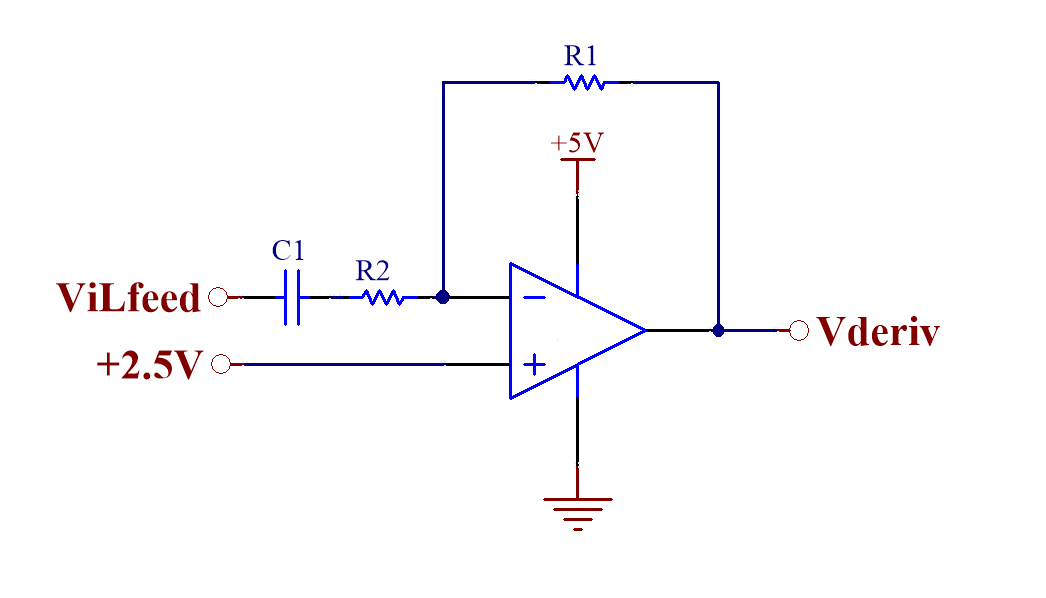
\includegraphics[scale=0.6]{Circuito-derivador- compensado.png}
	\caption{Circuito derivador compensado}
	\label{fig:img_Circuito_derivador_compensado}
\end{figure}

El operacional es internamente compensado, por lo que todos sus otros polos los tiene luego del cruce por $0\:dB$ de la ganancia. Para simplificar el análisis estos no se tienen en cuenta, ya que están fuera de la zona de interés.

\begin{equation} \label{eq_Aw_1}
	A(w)=\frac{1778279}{(\frac{s}{2\pi *20}+1)}
\end{equation} 

\begin{equation} \label{eq_Aw_2}
	\frac{1}{H(w)}=\frac{1+s*C_1*(R_1+R_2)}{1+s*C_1*R_2}\simeq \frac{1+s*C_1*R_1}{1+s*C_1*R_2}
\end{equation}

Para compensar el circuito se coloca un polo en $16 \:kHz$, que da como resultado $R_2=10\:\Omega$, $C_1=1\:uF$ y $R_1=25\: k\Omega$ y un margen de fase de $\phi =49.6{}^\circ $, como se puede observar en la figura \ref{fig:img_GH del derivador compensado}.

\begin{figure}[H]
	\centering
	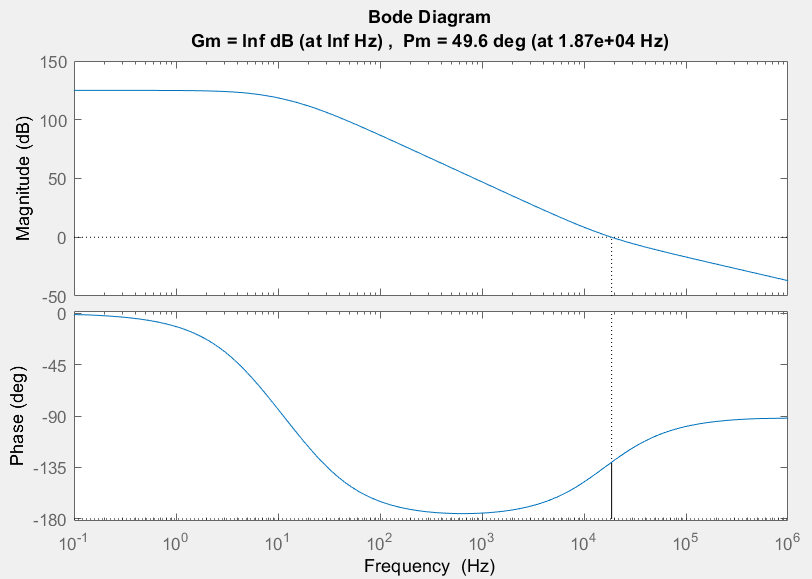
\includegraphics[scale=0.5]{GH-del-derivador-compensado.png}
	\caption{Transferencia a lazo abierto del derivador compensado.}
	\label{fig:img_GH del derivador compensado}
\end{figure}

\begin{figure}[H]
	\centering
	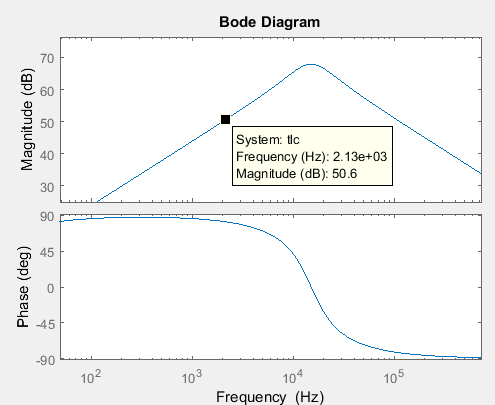
\includegraphics[scale=0.7]{Transferencia-de-lazo-cerrado.png}
	\caption{Transferencia de lazo cerrado.}
	\label{fig:img_Transferencia-de-lazo-cerrado}
\end{figure}

Como se observa en la figura \ref{fig:img_Transferencia-de-lazo-cerrado}, la transferencia de lazo cerrado (TLC) tiene un comportamiento derivativo en las frecuencias cercanas a $2 \:kHz$, como es deseado.

A continuación se muestra la TLC del circuito derivador:

\begin{equation} \label{eq_TLC_derivador}
	{TLC}_{derivador}=\frac{V_{yf}}{V_{iL}}=\frac{-0.025*s}{1+(\frac{2*0.473}{94.5\: k})*s+(\frac{s}{94.5\:k})^2}
\end{equation} 
ñ
\section{Diseño del filtro pasa bajos}

Debido a que el derivador amplifica las señales de alta frecuencia es necesario agregar un filtro pasa bajos en su entrada. Como la señal que ingresa al derivador es $V_{iL}$, que es una onda triangular de frecuencia fundamental de $2\:kHz$, se permite el paso de sus componentes hasta la 5º armónica. Para su implementación se utiliza un filtro activo Butterworth de segundo orden, con una frecuencia de corte en $20\:kHz$. En la figura  \ref{fig:img_Filtro-para-la-entrada-del-derivador} se puede ver el filtro utilizado y en la figura \ref{fig:img_Respuesta-en-frecuencia-del-filtro-activo}, su respuesta en frecuencia.

\begin{figure}[H]
	\centering
	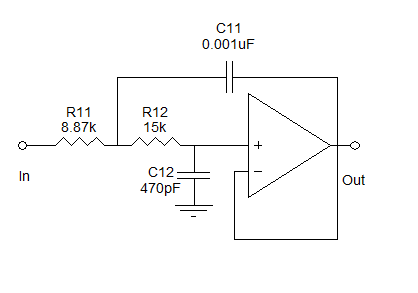
\includegraphics[scale=0.70]{Filtro-para-la-entrada-del-derivador.png}
	\caption{Filtro para la entrada del derivador.}
	\label{fig:img_Filtro-para-la-entrada-del-derivador}
\end{figure}

\begin{figure}[H]
	\centering
	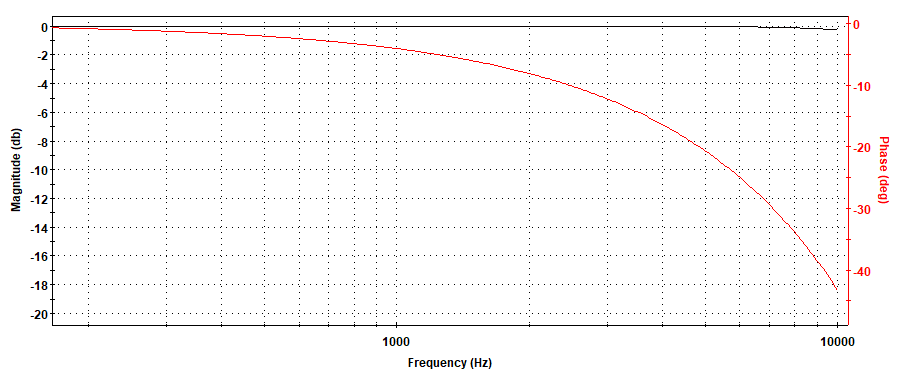
\includegraphics[scale=0.45]{Respuesta-en-frecuencia-del-filtro-activo.png}
	\caption{Respuesta en frecuencia del filtro activo.}
	\label{fig:img_Respuesta-en-frecuencia-del-filtro-activo}
\end{figure}

\section{Compensación de resistencia interna}

Al circular corriente siempre en el mismo sentido por el electroimán, se produce una caída de tensión casi constante en su resistencia interna. Esto provoca que no siempre estén aplicados $\pm 24\:V$ al electroimán sino que, durante el $T_{ON}$ se aplican $+24\:V-I_L*R_L$ y durante el $T_{OFF}$ se aplican $-24\:V-I_L*R_L$. Esto genera que las pendientes sean distintas.

\begin{equation} \label{eq_Vbus-didt-RL}
	\pm V_{BUS}-L(Y_g)*\left|\frac{{dI}_L}{dt}\right|-L_{\infty }*\left|\frac{{dI}_L}{dt}\right|-R_L*I_L=0
\end{equation}

Con  $R_L=0.2 \:\Omega$ y una corriente nominal  de aproximadamente $21\:A$:

\begin{equation} \label{eq_Vbus-didt-RL-2}
	\pm V_{BUS}-R_L*I_L=\ \pm 24\:V-4.2\:V
\end{equation}

Para el caso en que $V_{BUS}=24\:V$:

\begin{equation} \label{eq_Vbus-didt-RL-3}
	V_{BUS}-R_L*I_L=\ +24\:V-4.2\:V=\ 19.8\:V
\end{equation}

Para el caso en que $V_{BUS}=-24\:V$:

\begin{equation} \label{eq_Vbus-didt-RL-4}
	V_{BUS}-R_L*I_L=\ -24\:V-4.2\:V=\ 28.2\:V
\end{equation}

Por lo tanto, sobre el electroimán se aplican dos tensiones distintas, en valor absoluto, durante la carga y descarga. Esto provoca que la rampa de corriente sea asimétrica.

Debido a que luego se utilizará un rectificador de onda completa, se desea que la rectificación de cada una de estas pendientes resulte en el mismo valor. En la figura \ref{fig:img_Forma-de-onda-luego-de-rectificar-sin-compensación-IR} se muestra el efecto luego de la rectificación sin realizar ninguna compensación.

\begin{figure}[H]
	\centering
	\includegraphics[scale=0.8]{Forma-de-onda-luego-de-rectificar-sin-compensación-IR.png}
	\caption{Forma de onda luego de rectificar sin compensación de resistencia interna.}
	\label{fig:img_Forma-de-onda-luego-de-rectificar-sin-compensación-IR}
\end{figure}

Para corregir este problema, se varía \textsl{set-point} de la salida del derivador. Para lograrlo se debe cambiar la tensión en la entrada no inversora ($V_{bias}$) como se muestra en la figura \ref{fig:img_Esquema-circuital-del-derivador}. 

\begin{figure}[H]
	\centering
	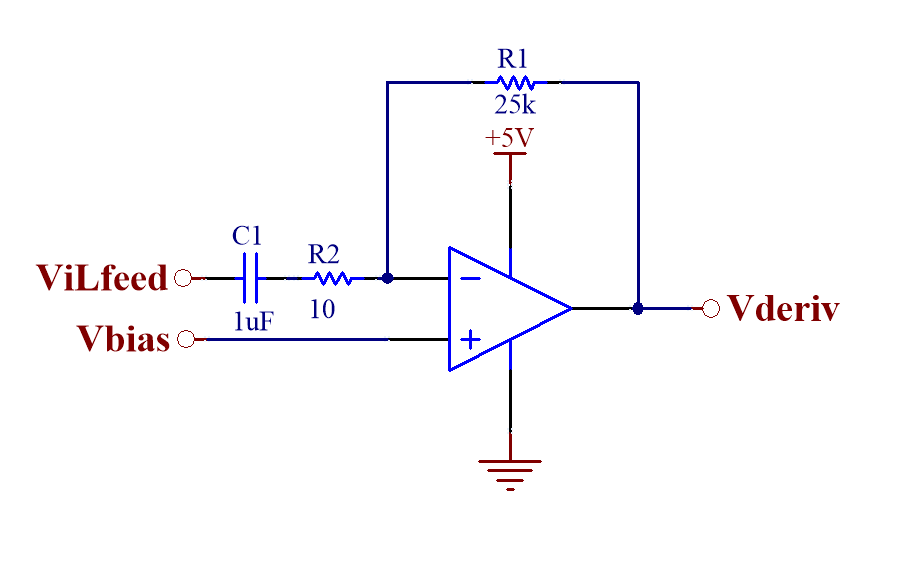
\includegraphics[scale=0.6]{Esquema-circuital-del-derivador.png}
	\caption{Esquema circuital del derivador con $V_{bias}$.}
	\label{fig:img_Esquema-circuital-del-derivador}
\end{figure}

Se tiene que la pendiente de bajada de la onda triangular, en módulo, es mayor que la de subida. Por lo tanto, al derivarla (con la inversión de signo), queda por encima del \textsl{set-point}, y la pendiente de subida, por debajo. Por ello, se debe compensar el \textsl{set-point} para que la forma de onda sea simétrica alrededor de $2.5\:V$. 

Para la pendiente de bajada, la salida del derivador es:

\begin{equation} \label{eq_Vyf-Vbias}
	{Vyf}_{off}\ =\ V_{bias}+K_h\ *\ \tau *\frac{\abs{V_{BUS}}\ +\ I_L*R_L}{L}\ 
\end{equation}

Para la pendiente de subida se tiene:

\begin{equation} \label{eq_Vyf-Vbias2}
	{Vyf}_{on}\ =\ V_{bias}\ -\ K_h\ *\ \tau *\frac{\abs{V_{BUS}} -\ I_L*R_L}{L}
\end{equation}

Se desea que se cumpla:

\begin{equation} \label{eq_Vyf_Vbias3}
	{Vyf}_{off}\ -2.5\ \:V=\ 2.5\ V\ -{Vyf}_{on}
\end{equation}

Si se despeja $V_{bias}$ se llega a:

\begin{equation} \label{eq_Vyf-Vbias4}
	V_{bias}\ =2.5\ \:V -\ K_h\ *I_L*\ \tau *\frac{\ R_L}{L}
\end{equation}

Se tiene $K_h = 53.3\:\frac{mV}{A},\; R_L = 0.2\:\Omega$ y $\tau  = 25 \:ms$. En cuanto a la inductancia, se utiliza:  $L_T(4\:mm) = 16.44\:mHy$.

$V_{iL}$ es la tensión de salida del sensor de efecto Hall menos un \textsl{set-point} de $2.5\:V$. Sin embargo, debido al \textsl{offset} agregado al sensor para llevar su valor medio a $2.6\:V$, al restarle $2.5\:V$ no se produce una cancelación completa sino que quedan $0.1\:V$ de error. Por ello, para implementar la ecuación  \ref{eq_Vyf_Vbias3} se utiliza el circuito mostrado en la figura \ref{fig:img_Generación_de_Vbias}. Este circuito compensa la diferencia de pendientes, el error de $0.1\:V$ y genera $V_{bias}$ para ingresar al derivador.

\begin{figure}[H]
	\centering
	\includegraphics[scale=0.6]{Generación-de-Vbias.png}
	\caption{Generación de $V_{bias}$.}
	\label{fig:img_Generación_de_Vbias}
\end{figure}

A partir del circuito de la figura \ref{fig:img_Generación_de_Vbias} se obtiene:

\begin{equation} \label{eq_Vyf-Vbias3}
	V_{bias} =-\frac{R_4}{R_3}(K_hI_L+ 0.1\:V)+V_{Ref_{bias}}(1+\frac{ R_4}{R_3})(\frac{R_1}{R_1+R_2})
\end{equation}

Para poder llegar a la expresión de la ecuación \ref{eq_Vbus-didt-RL-2} se debe cumplir que:

\begin{enumerate}
	\item  $-\frac{R_4}{R_3}=- \tau *\frac{R_L}{L}= -0.304$  
	
	\item  $-\frac{R_4}{R_3}(0.1V)+V_{Ref_{bias}}(1+\frac{ R_4}{R_3})(\frac{R_1}{R_1+R_2}) = 2.5V$     
\end{enumerate}

Por lo tanto, al resolver la condición 1) se elige $R_4 = 304\: \Omega$ y se obtiene $R_3=1\:k\Omega$. Luego, al resolver la condición 2) con $V_{Ref_{bias}}=2.5\:V$ se elige $R_1=1\:k\Omega$ y se obtiene $R_{2}=291.8\:\Omega$.

En la figura \ref{fig:img_Formas_de_onda_obtenidas_en_la_simulación} se muestra como cambia la forma de onda.

\begin{figure}[H]
	\centering
	\includegraphics[scale=0.6]{Formas-de-onda-obtenidas-en-la-simulación.png}
	\caption{Formas de onda obtenidas en la simulación.}
	\label{fig:img_Formas_de_onda_obtenidas_en_la_simulación}
\end{figure}

La onda superior corresponde a la corriente en el electroimán, la que se encuentra al medio, a la salida del derivador y la inferior, a la onda rectificada con la corrección de la resistencia interna.

\section{Rectificación y suavizado}

Para poder tener finalmente la estimación de la posición, se debe rectificar la salida del derivador alrededor de $2.5\:V$. Esto se hace para que la pendiente positiva de la corriente triangular coincida con la pendiente negativa, y tener a la salida del estimador una señal aproximadamente continua.

En la figura \ref{fig:img_Circuito_estimador_de_posición_completo} se puede observar el circuito completo utilizado para la implementación de la rectificación y filtrado. Para facilitar la comprensión de esta última parte del estimador, se realiza un análisis de cada una de estas etapas por separado.

\begin{figure}[H]
	\centering
	\includegraphics[scale=0.5]{Circuito-estimador-de-posición-completo.png}
	\caption{Circuito de rectificación, resta y filtrado.}
	\label{fig:img_Circuito_estimador_de_posición_completo}
\end{figure}

\subsection{Rectificador}

Para entender el funcionamiento de este rectificador, se comienza con el análisis de la primer etapa del circuito de la figura \ref{fig:img_Circuito_estimador_de_posición_completo}. Por lo tanto, se simplifica el circuito al mostrado en la figura \ref{fig:img_Rectificador_y_restador}. Se parte de la suposición de que en un amplificador ideal, la tensión diferencial ($V_d$) es igual a cero. De esta forma, como la entrada no inversora está fijada en $2.5\:V$, la misma tensión se encuentra en la entrada inversora.


\begin{figure}[H]
	\centering
	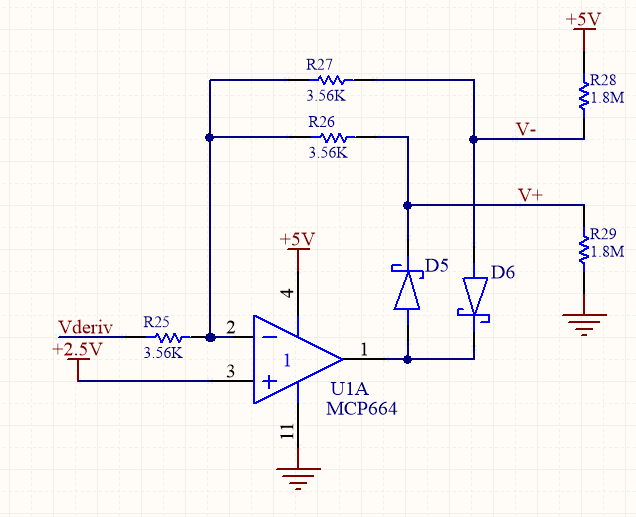
\includegraphics[scale=0.7]{Rectificador-y-restador.png}
	\caption{Circuito rectificador.}
	\label{fig:img_Rectificador_y_restador}
\end{figure}

Al analizar la corriente en la resistencia $R_{25}$ (con sentido positivo hacia la izquierda) en función de $V_{deriv}$, resulta:

\begin{equation} \label{eq_corriente_r25}
	I_{R25}=\frac{2.5\:V\ -\ V_{deriv}}{R_{25}}
\end{equation}

En el caso de que $V_{deriv}$ $\mathrm{<}$ $2.5\:V$, la corriente será positiva. Esta misma corriente proviene desde la salida del operacional, a través del diodo $D_5$ y la resistencia $R_{26}$. Si se desprecia la tensión del diodo en directa se obtiene que la salida del operacional es igual a $V^+$:

\begin{equation} \label{eq_V+}
	V^+=I_{R25}*R_{26}+2.5\:V=\frac{2.5\:V-V_{deriv}\ }{R25}*R_{26}+2.5\:V\ 
\end{equation} 

Como $R_{25}=R_{26}$

\begin{equation} \label{eq_V+_2}
	V^+\ =\ 2.5\:V\ -\ V_{deriv}\ +2.5\:V\ =\ 5\:V\ -\ V_{deriv}\ 
\end{equation}

Además, dado que el diodo $D_6$ queda polarizado en inversa y la caída de tensión en $R_{27}$ es despreciable, se obtiene que $V^- = 2.5\:V$.

Análogamente, si $V_{deriv}$ $\mathrm{>}$ $2.5\:V$, se puede encontrar:

\begin{equation} \label{eq_V+_3}
	V^- =5\:V-V_{deriv} 
\end{equation}

\begin{equation} 
	V^+ = 2.5\:V
\end{equation}


\subsection{Restador}

Se utiliza un amplificador operacional en modo diferencial como restador. El circuito utilizado se observa en la figura \ref{fig:img_Restador} y se obtiene lo siguiente:

Cuando $V_{deriv}$ $\mathrm{<}$ $2.5\:V$:
\begin{equation*} 
	\begin{aligned}
		V_{estim}&=V^+-\ V^-\ +2.5\:V\\ 
		V_{estim}&=(5\:V -\ V_{deriv})-(2.5\: V)+2.5\:V\\
		V_{estim}&=5\: V\ -\ V_{deriv}\\ 
	\end{aligned}
\end{equation*}


Cuando $V_{deriv}$ $\mathrm{>}$ $2.5\:V$: 
\begin{equation*} 
	\begin{aligned}
		V_{estim}&=V^+-\ V^-+2.5V\\ 
		V_{estim}&=2.5V\ -\ (5V-\ V_{deriv})+\ 2.5V\\
		V_{estim}&=V_{deriv}\\
	\end{aligned}
\end{equation*}

Si se toma a $V_{deriv}$ como $V_{deriv}=\mathit{\Delta}V_{deriv}\ +\ 2.5\: V$, al reemplazar en los dos casos se obtiene:
\begin{equation} \label{eq_rest_3}
	V_{estim}= 2.5\:V + |\mathit{\Delta}V_{deriv}|
\end{equation}

\begin{figure}[H]
	\centering
	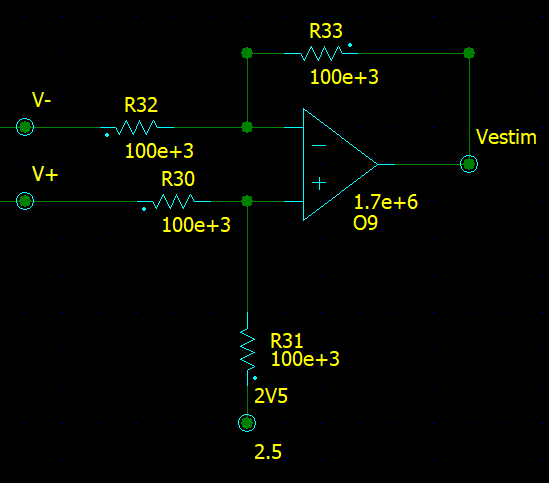
\includegraphics[scale=0.7]{Restador.png}
	\caption{Circuito restador.}
	\label{fig:img_Restador}
\end{figure}

\subsection{Filtrado}

En el restador se implementa un filtrado adicional a la señal de salida como se observa en la figura  \ref{fig:img_Esquema-circuital-del-restador-con-una-etapa-de-filtrado-en-159}. De esta \'{u}ltima etapa, si se considera $C_5=C_6=C\ $y $R_{33}=R_{31}=R$, se obtiene:



\begin{equation}
	V_{estim}=\frac{1}{1+s*C*R}*{(V}^+-V^-\ +\ 2.5\:V)
\end{equation}

\begin{equation} \label{eq_Vestim_1}
	V_{estim}=\frac{1}{1+s*C*R}*(2.5\: V\ +\ |\mathit{\Delta}V_{deriv}|)
\end{equation}

\begin{equation} \label{eq_Vestim_2}
	V_{estim} \approx \frac{1}{1+s*C*R}*\ |\mathit{\Delta}V_{deriv}|\ +2.5\:V
\end{equation}



Puesto que la salida $V_{estim}$ debe ser una continua, es importante eliminar cualquier posible ripple. Por ello, se escogen los siguientes valores para los componentes:

\begin{enumerate}
	\item  $C=10\: nF$
	
	\item  $R=100\:\Omega$
	
	\item  $\frac{1}{2*\pi *C*R}=159.2\: Hz$
\end{enumerate}

\begin{figure}[H]
	\centering
	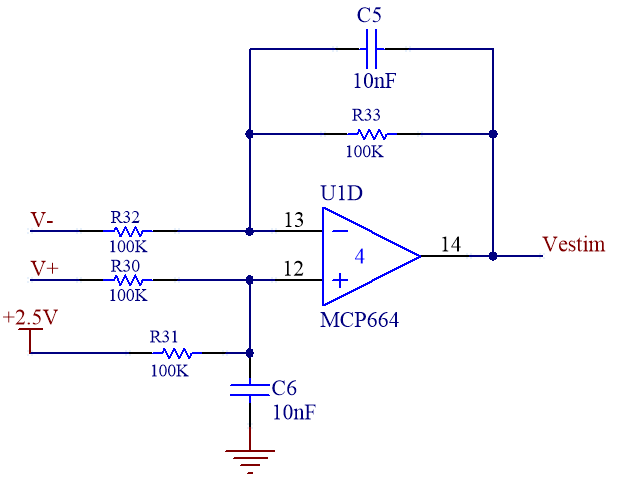
\includegraphics[scale=0.7]{Esquema-circuital-del-restador-con-una-etapa-de-filtrado-en-159.png}
	\caption{Esquema circuital del restador con una etapa de filtrado en $159.2\: Hz$.}
	\label{fig:img_Esquema-circuital-del-restador-con-una-etapa-de-filtrado-en-159}
\end{figure}

\section{Simulación del estimador completo}

En la figura \ref{fig:img_Simulación_final_del_estimado} se pueden observar tres formas de onda. La superior corresponde a la corriente del electroimán, la del medio a la salida del derivador y la inferior a la salida $V_{estim}$. Con el uso de los cursores se midió un ripple de $52.66\:mV $ en $V_{estim}$.

\begin{figure}[H]
	\centering
	\includegraphics[scale=0.6]{Simulación-final-del-estimador.png}
	\caption{Simulación final del estimador.}
	\label{fig:img_Simulación_final_del_estimado}
\end{figure}

En la tabla \ref{tab_Resultados_de_simulación_del_estimador} se muestran valores medidos de $V_{estim}$ en función de la posición.

\begin{table}[H]
	\begin{center}
		\begin{tabular}{| c | c | c |}
			\hline
			$Y_g\:[mm]$ & $L(Y_g)\:[mHy]$ & $V_{estim}\:[V]$ \\ \hline 
			2 & 22.64 & 3.86 \\ \hline 
			3 & 18.8 & 4.13 \\ \hline 
			4 & 16.44 & 4.36 \\ \hline 
			5 & 14.9 & 4.55 \\ \hline 
		\end{tabular}
		\caption{Resultados de simulación del estimador.}
		\label{tab_Resultados_de_simulación_del_estimador}
	\end{center}
\end{table}

\section{Transferencia final del estimador de posición}

El funcionamiento del circuito estimador no es lineal.  Por lo tanto, para poder modelar una función transferencia, se deben tomar ciertas consideraciones. La parte del derivador es lineal, por lo que se puede modelar su transferencia como:
\begin{equation}\label{eq_v-estim}
	V_{estim}=-0.025*\frac{dVi_L}{dt} 
\end{equation}

A partir de la expresión \ref{eq_v-estim} se puede determinar que, además de realizarse la derivada, se introduce una inversión de signo. De esta forma, una pendiente positiva a la entrada resulta en valores menores a $2.5\:V$ a la salida, mientras que una pendiente negativa produce una tensión mayor a $2.5\:V$.

Luego, el bloque rectificador y restador se encarga de calcular el valor absoluto de esta señal (en torno a los $2.5\:V$). Al considerar que la pendiente aumenta a medida que lo hace la distancia de separación, se puede concluir que el bloque estimador no produce inversión de signo. Por lo tanto, se debe considerar solamente la ganancia del derivador y el polo que introduce la etapa de restador. Finalmente, para poder obtener una estimación de la posición, se utiliza la expresión linealizada \ref{eq_di-dt_lineal} que relaciona la derivada de la corriente con el entrehierro:

\begin{equation} \label{eq_dil_yg}
	\frac{dI_{L}}{dt} = 194690 * Y_{g}
\end{equation}


Al considerar la ganancia que tiene el sensor de efecto Hall sobre la corriente:

\begin{equation} \label{eq_dil_dvil}
	\frac{dI_{L}}{dt} =\frac{dVi_{L}}{dt}*\frac{1}{0.0533}
\end{equation}

Por lo tanto al utilizar \ref{eq_dvil_yg} en \ref{eq_dil_yg} se obtiene \ref{eq_dvil_yg}.

\begin{equation} \label{eq_dvil_yg}
	\frac{dVi_{L}}{dt} = 0.0533*194690*Y_{g}
\end{equation}


En base al resultado anterior, se llega a:



\begin{equation}
	V_{estim}=0.025*194690*0.0533 * \frac{Y_{g}}{1 + \frac{s}{1\:k}}=259.6*\frac{Y_{g}}{1 + \frac{s}{1\:k}}	
\end{equation}

Finalmente, al considerar la etapa de filtrado de la entrada, que tiene dos polos en $2\pi *10\: \:{kHz}\ \simeq 60\: \:{krad/s}$ se obtiene:

\begin{equation} \label{eq_TLC_deriv_7}
	H_{estim}=\frac{V_{estim}}{Y_{g}[m]}=\frac{259.6}{(1+\frac{s}{1\:k})*{(1+\frac{s}{60\: k})}^2}
\end{equation}

